\documentclass[12pt, a4paper]{article}

\usepackage{lipsum}% http://ctan.org/pkg/lipsum
\setlength{\parindent}{1.25cm}

\usepackage{hyperref}
\hypersetup{
    colorlinks=true, % make the links colored
    linkcolor=black, % color TOC links in blue
    urlcolor=red, % color URLs in red
    linktoc=all % 'all' will create links for everything in the TOC
}
\usepackage{mathtext}
\usepackage[T2A]{fontenc}  % поддержка кириллицы в ЛаТеХ
\usepackage[utf8]{inputenc} % кодировка
\usepackage[english, russian]{babel} % определение языков в документе
% \usepackage{pscyr} % красивые кириллические шриф ты
% \usepackage{mathspec}
% \usepackage{upgreek} % добавляет прямые греческие символы
\usepackage[eulergreek, italic]{mathastext}
% \usepackage{lscape} % для включения альбомных страниц (широкие таблицы, графики и т.д.)

% \usepackage{nath}

\usepackage{amsmath} % многострочные формулы
% \usepackage{breqn}  % автоматические многострочные формулы
\usepackage{amstext} % определяет \textit{} для включения в формулы текста
\usepackage{amssymb} % набор символов
% \usepackage{makecell} % работа с ячейками в таблицах
% \usepackage[math-style=upright]{unicode-math}
\usepackage{indentfirst}  % делает отступ в начале параграфа

% \usepackage{lmodern}
% \usepackage{listings} % для листингов программ
\usepackage{pdflscape} % альбомные страницы

\usepackage{longtable} % для многостраничных таблиц
\usepackage{multirow}  % для объединения ячеек таблиц
\usepackage{multicol}  % для объединения ячеек таблиц

\usepackage{mathtools}
% \usepackage{makeidx}
% \usepackage{amssymb}
% \usepackage{amsfonts}
\usepackage{cite}
% \usepackage{hyperref}

\usepackage{enumerate} % нумерация списков
\usepackage{enumitem}

% \usepackage{txfonts}
% \usepackage{kpfonts}

% \usepackage{float}
% \usepackage{mathdots}
% \usepackage{pdflscape}
\usepackage{array}

\pagestyle{empty}

% \usepackage{ltxtable}
% \usepackage{lipsum}

\usepackage{geometry} % размеры листа
\geometry{left = 3cm} % размеры листа
\geometry{right = 2cm} % размеры листа
\geometry{top = 2cm} % размеры листа
\geometry{bottom = 2cm} % размеры листа

\usepackage[figurename=Рисунок]{caption}
\usepackage{subcaption}

\DeclareCaptionLabelFormat{continued}{Продолжение таблицы~#2}
\DeclareCaptionLabelFormat{gostfigure}{Рисунок #2}
\DeclareCaptionLabelFormat{gosttable}{Таблица #2}
\DeclareCaptionLabelSeparator{gost}{~---~}

\captionsetup[figure]{justification = centering}
\captionsetup{labelsep=gost}
\captionsetup*[figure]{labelformat=gostfigure}

\usepackage{graphicx}
% \setlength\extrarowheight{6pt}

\renewcommand{\rmdefault}{ftm} % переключение на общий шрифт документа Times New Roman (пакет pscyr)
%\renewcommand\theadfont{\normalsize}

\linespread{1.3}

\frenchspacing

% \usepackage{tikz}
% \usetikzlibrary{shapes.geometric, arrows}
% \usetikzlibrary{automata,positioning}


\usepackage{titlesec}

% Настройка формата разделов и подразделов
\titleformat{\section}{\normalfont\normalsize\bfseries}{\thesection}{1em}{}
\titleformat{\subsection}{\normalfont\normalsize\bfseries}{\thesubsection}{1em}{}
\titleformat{\subsubsection}{\normalfont\normalsize\bfseries}{\thesubsubsection}{1em}{}

% Настройка расстояния до разделов и подразделов и после
\titlespacing*{\section}{\parindent}{0pt}{18pt}
\titlespacing*{\subsection}{\parindent}{18pt}{18pt}
\titlespacing*{\subsubsection}{\parindent}{18pt}{18pt}

% Каждый раздел с новой страницы
\newcommand{\sectionbreak}{\clearpage}

% \addto\captionsenglish{
% \renewcommand\contentsname{СОДЕРЖАНИЕ}
% }
\addto\captionsrussian{
    \renewcommand\contentsname{\hfill СОДЕРЖАНИЕ\hfill}
}

%\usepackage{accsupp}

\makeatletter
\renewcommand*\l@section{\@dottedtocline{1}{1.5em}{2.3em}}
\renewcommand*\l@subsection{\@dottedtocline{1}{1.5em}{2.3em}}
\renewcommand*\l@subsubsection{\@dottedtocline{1}{1.5em}{2.3em}}
% \newcommand\cdot {\copyable}{%
%   \begingroup
%   \@sanitize
%   \catcode`\%=14 % allow % as comment char, also needed for \%
%   \@copyable
% }
% \newcommand\cdot {\@copyable}[1]{%
%   \endgroup
%   \BeginAccSupp{%
%     ActualText=\detokenize{#1},%
%     method=escape,
%   }%
%   \scantokens{#1}%
%   \EndAccSupp{}%
% }
\makeatother


\begin{document}

\begin{titlepage}

\begin{center}
Министерство образования и науки Российской Федерации\\
Федеральное государственное автономного образовательное учреждение высшего образования\\
\hrulefill\\
\vspace{0.5cm}
САНКТ-ПЕТЕРБУРГСКИЙ ПОЛИТЕХНИЧЕСКИЙ УНИВЕРСИТЕТ\\ ПЕТРА ВЕЛИКОГО\\
\vspace{0.5cm}
Институт Энергетики\\
Высшая школа энергетического машиностроения\\

\end{center}

\vspace{5cm}
\begin{center}
\begin{large}
Лабораторная работа №1 \\
"Определение собственных частот колебаний ротора с диском"
\end{large}
\end{center}

\vspace{5cm}
\hspace{5cm} Студент гр. 3231303/81001 \hrulefill Степанов С.С.


\vspace{0.5cm}
\hspace{5cm} Преподаватель \hrulefill Курнухин А.А. \\


\vfill
\begin{center}
Санкт-Петербург\\
2021
\end{center}

\end{titlepage}

\tableofcontents
\newpage

\section{Теория}
При проектировании газотурбинных двигателей рассматриваются такие явления, которые связаны с большими частотами вращения упругих роторов ГТД и взаимодействием роторных систем с упругим корпусом. По мере приближения частоты вращения вала к критической происходит потеря устойчивости быстровращающихся роторов, что ведет к резонансным режимам системы ротор – корпус. Эти явления сопряжены с опасностью выхода из строя элементов конструкции, приводящему к разрушению двигателя.\\

\begin{figure}[h]
\center
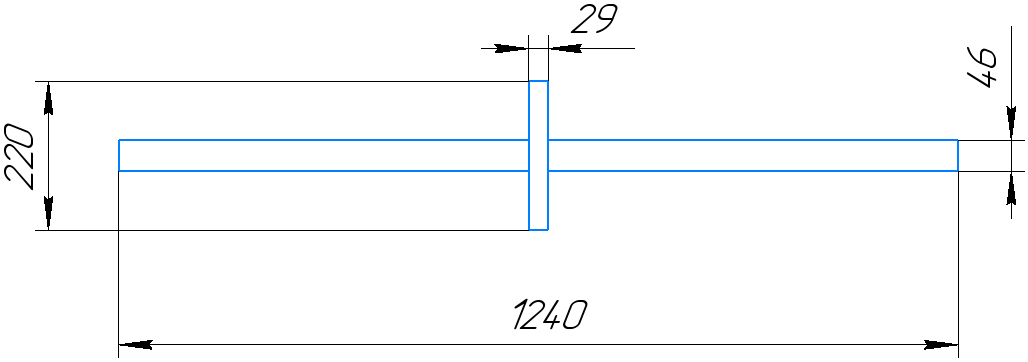
\includegraphics[width=120mm]{rotor.png}
\caption{Чертеж ротора с диском} \label{fig:1}
\end{figure}

В ходе данной лабораторной работы были произведены расчеты собственных частот колебаний ротора с диском при различных условиях закрепления, а так же расчет собственных частот крутильных колебаний.  

\section{Исходные данные}

Длина ротора, [м]

\[l = 1,24.\]

Диаметр ротора, [мм]

\[d = 46\cdot10\textsuperscript{-3}.\]

Диаметр диска, [мм]

\[D = 220\cdot10\textsuperscript{-3}.\]

Толщина диска, [мм]

\[h = 29\cdot10\textsuperscript{-3}.\]

Плотность стали, [кг/м\textsuperscript{3}]

\[\rho = 8000.\]

Модуль упругости, [Па]
\[Е = 2\cdot10\textsuperscript{11}.\]


\section{Определение собственной частоты поперечных колебаний ротора с диском, расположенным между опорами}

Масса диска, [кг]

\[m = \rho\cdot V = \rho\cdot\frac{\pi\cdot D^{2}}{4} \cdot h = 8000\cdot\frac{3,14\cdot({220\cdot10^{- 3})}^{2}}{4}\cdot29\cdot10^{- 3} = 8,81.\ \]

Полярный момент инерции, [ м\textsuperscript{4}]

\[Y_{\textit{xx}} = \frac{\pi\cdot d^{4}}{64} = \frac{3,14\cdot({46\cdot10^{- 3})}^{4}}{64} = 2,19\cdot10^{-7}.\ \]

Податливость, [м/Н]

\[\delta_{11} = \frac{P\cdot {(2\cdot l)}^{3}}{48\cdot E\cdot Y_{\textit{xx}}} = \frac{1\cdot{(2\cdot1,24)}^{3}}{48\cdot2\cdot10^{11}\cdot2,197\cdot10^{- 7}} = 7,22\cdot10^{-6}.\ \ \]

Собственная частота поперечных колебаний, [Гц]

\[p = \sqrt{\frac{1}{\delta_{11}\cdot m}} = \sqrt{\frac{1}{7,232\ \cdot10^{- 6}\cdot8,81}} = 125,3\ \frac{рад}{с} = 19,93.\ \]

\[\]

\section{Определение собственных частот поперечных колебаний для консольного расположения диска}

Масса диска, [кг]

\[m = \rho\cdot V = \rho\cdot\frac{\pi\cdot D^{2}}{4}\cdot h = 8000\cdot\frac{3,14\cdot({220*10^{- 3})}^{2}}{4}\cdot29\cdot10^{- 3} = 8,81.\ \]

Полярный момент инерции, [ м\textsuperscript{4}]

\[Y_{x0} = \frac{\pi\cdot d^{4}}{64} = \frac{3,14\cdot({46\cdot10^{- 3})}^{4}}{64} = 2,19\cdot10^{-7}.\ \]

Податливость, [м/Н]

\[\delta_{11} = \frac{l^{3}}{3\cdot E\cdot Y_{x0}} = \frac{{1,24}^{3}\ }{3\cdot2\cdot10^{11}\cdot2,197\cdot10^{- 7}} = 1,4\cdot10^{-5}.\ \]

Собственная частота поперечных колебаний, [Гц]

\[p = \sqrt{\frac{1}{\delta_{11}\cdot m}} = \sqrt{\frac{1}{14,46\cdot10^{- 6}\cdot8,81}} = 88,6\ \frac{рад}{с} = 14,09.\ \]

а) С учётом момента инерции диска

Составим и решим систему уравнений:

\[\left\{ \begin{matrix}
y = \delta_{11}\cdot\left( - m\cdot\ddot{y} \right) + \delta_{12}\cdot( - \theta_{x}\cdot\ddot{\varphi}) \\
\varphi = \delta_{21}\cdot\left( - m\cdot\ddot{y} \right) + \delta_{22}\cdot( - \theta_{x}\cdot\ddot{\varphi}) \\
\end{matrix} \right.\ \]

\[y = Ye^{\textit{ipт}};\ \varphi = Фe^{\textit{ipт}}.\]

\[\left\{ 
\begin{matrix}
0 = \left( m\cdot p^{2}\cdot \delta_{11} - 1 \right)\cdot Y + \theta_{x}\cdot p^{2}\cdot\delta_{12}\cdot Ф \\
0 = m\cdot p^{2}\cdot \delta_{21}\cdot Y + {(\theta}_{x}\cdot p^{2}\cdot\delta_{22} - 1)\cdot Ф \\
\end{matrix} 
\right.\ \]

\[0 = \left| \frac{m\cdot p^{2}\cdot\delta_{11}\textit{\ \ \ \ }\theta_{x}\cdotp^{2}\cdot\delta_{12}}{m\cdot p^{2}\cdot\delta_{21}\textit{\ \ \ }\theta_{x}\cdot p^{2}\cdot\delta_{22}\ } \right|\]

\[p^{4}\cdot m\theta_{x}\cdot\left( \delta_{11}\cdot\delta_{22} - \delta_{12}\cdot\delta_{21} \right) - p^{2}\cdot{(\theta}_{x}\cdot\delta_{22} + m\cdot\delta_{11}) + 1 = 0.\]

Податливость, [м/Н]

\[\delta_{11} = \frac{l^{3}}{3\cdot E\cdot Y_{x0}} = \frac{{1,24}^{3}}{3\cdot2\cdot10^{11}\cdot2,297\cdot10^{- 7}} =1,44\cdot10^{-5};\ \]


\[\delta_{21} = \delta_{12} = \frac{l^{2}}{2\cdot E\cdot Y_{x0}} = \frac{{1,24}^{2}}{2\cdot2\cdot10^{11}\cdot2,179\cdot10^{- 7}} = 1,75\cdot10^{-5};\ \]


\[\delta_{22} = \frac{l}{E\cdot Y_{x0}} = \frac{1,24}{2\cdot10^{11}\cdot2,197\cdot10^{- 7}} = 2,82\cdot10^{-5}.\ \]

Момент инерции, [кг $\cdot$ м\textsuperscript{2}]

\[\theta_{x} = \frac{m\cdot\left( \frac{D}{2} \right)^{2}}{2} = \frac{8,81\cdot\left( \frac{220\cdot10^{- 3}}{2} \right)^{2}}{2} = 0,053;\ \]

Получим квадратное уравнение:

\[4,783\cdot10^{- 11}р^{4} - 1,289\cdot10^{- 4}р^{2} + 1 = 0;\]

Дискриминант:

\[Д = \left( - 1,289\cdot10^{- 4} \right)^{2} - 4\cdot4,783\cdot10^{- 11}\cdot1 = 16,43\cdot10^{- 9}.\]

Корни уравнения:

\[р^{2} = \frac{1,289\cdot10^{- 4} - \sqrt{16,43\cdot10^{- 9}}}{2\cdot4,783\cdot10^{- 11}} = 7773;\]

\[р^{2} = \frac{1,289\cdot10^{- 4} + \sqrt{16,43\cdot10^{- 9}}}{2\cdot4,783\cdot10^{- 11}} = 2681210.\]

Собственные частоты колебаний, [Гц]

\[p  = 88,17;\ \]

\[p  = 1637,44.\ \]

Проверка ортогональности:

\[Y_{1} = 1;\ Y_{2} = 1.\]

\[Ф_{1} = \frac{1 - m\cdotр_{2}^{2}\cdot\delta_{11}}{\ \theta_{x}\cdot р_{2}^{2}\cdot\delta_{12}} = \frac{1 - 8,81\cdot{1639,3}^{2}\cdot14,46\cdot10^{- 6}}{53300\cdot10^{- 6}\cdot{1639,3}^{2}\cdot17,5\cdot10^{- 6}} = -136,239;\]

\[Ф_{2} = \frac{\ \theta_{x}\cdot р_{1}^{2}\cdot\delta_{21}}{\ 1 - m\cdot р_{1}^{2}\cdot\delta_{22}} = \frac{53300\cdot10^{- 6}\cdot{86,8}^{2}\cdot17,5\cdot10^{- 6}}{1 - 8,81\cdot{86,8}^{2}\cdot28,22\cdot10^{- 6}} = -0,007.\]

\[Y_{1}\cdot Y_{2}\cdot m + \theta_{x}\cdot Ф_{1}\cdot Ф_{2} = 8,87.\]

\section{Определение собственных частот крутильных колебаний}

Масса диска, [кг]

\[m = \rho\cdot V = \rho\cdot\frac{\pi\cdot D^{2}}{4}\cdot h = 8000\cdot\frac{3,14\cdot({220\cdot10^{- 3})}^{2}}{4}\cdot29\cdot10^{- 3} = 8,81.\ \]

Полярный момент инерции, [ м\textsuperscript{4}]

\[Y_{x0} = \frac{\pi\cdot d^{4}}{64} = \frac{3,14\cdot({46\cdot10^{- 3})}^{4}}{64} = 2,19\cdot10^{-7}.\ \]

Податливость, [м/Н]

\[\delta = \frac{l}{E\cdot Y_{x0}} = \frac{1,24}{2\cdot10^{11}\cdot2,197\cdot10^{- 7}} = 2,82\cdot10^{-5}.\ \]

Собственная частота колебаний, [Гц]

\[р = \sqrt{\frac{1}{\delta\cdot \textit{m}}} = \sqrt{\frac{1}{28,22\cdot10^{- 6}\cdot8,81}} = 63,42\ \frac{рад}{с} = 10,09.\ \]

\section{Определение характеристик затухания}

\[\frac{A_{i}}{A_{i + 1}} = \frac{12}{11};\]

\[\eta = \ln\frac{A_{i}}{A_{i + 1}} = \ln\frac{12}{11} = 0,087;\]

\[\beta = \frac{\eta}{\pi} = \frac{0,087}{3,14} = 0,0277.\]

\section{Список использованной литературы}

1. Костюк А.Г. Динамика и прочность турбомашин: Учебник для вузов.  Москва.: Издательский дом МЭИ, 2007. 477 с.

\end{document}
